\documentclass[a5paper]{article}
\usepackage[a5paper, top=8mm, bottom=8mm, left=8mm, right=8mm]{geometry}

\usepackage{polyglossia}
\setdefaultlanguage[babelshorthands=true]{russian}

\usepackage{fontspec}
\setmainfont{FreeSerif}
\newfontfamily{\russianfonttt}[Scale=0.7]{DejaVuSansMono}

\usepackage[font=scriptsize]{caption}

\usepackage{amsmath}
\usepackage{amssymb,amsfonts,textcomp}
\usepackage{color}
\usepackage{array}
\usepackage{hhline}
\usepackage{cite}

\usepackage[hang,multiple]{footmisc}
\renewcommand{\footnotelayout}{\raggedright}

\PassOptionsToPackage{hyphens}{url}\usepackage[xetex,linktocpage=true,plainpages=false,pdfpagelabels=false]{hyperref}
\hypersetup{colorlinks=true, linkcolor=blue, citecolor=blue, filecolor=blue, urlcolor=blue, pdftitle=1, pdfauthor=, pdfsubject=, pdfkeywords=}

\usepackage{tabu}

\usepackage{graphicx}
\usepackage{indentfirst}
\usepackage{multirow}
\usepackage{subfig}
\usepackage{footnote}
\usepackage{minted}

\tabulinesep=1.2mm

\sloppy
\pagestyle{plain}

\title{Язык программирования Java, введение}
\author{Юрий Литвинов\\\small{yurii.litvinov@gmail.com}}

\date{16.01.2019}

\begin{document}

\maketitle
\thispagestyle{empty}

\section{Формальности}

Занятия будут раз в неделю, две пары подряд. На занятиях я обычно буду что-то рассказывать (но немного, раз у вас есть хороший лекционный курс по Java), потом мы будем, собственно, практиковаться, решая прямо на паре несложные задачи, ну и у нас запланировано несколько пар лекционного формата. Однако основная практика будет в виде домашних заданий, которых будет много (поскольку единственный известный мне способ научиться программировать --- это много программировать, так же как нельзя научиться летать, читая книжки про самолёты). Кстати, я считаю, что учить собственно язык программирования нет особого смысла, потому что по Java полно хороших книг и читать все умеют, так что тратить время на парах на зачитывание вслух документации по языку и стандартной библиотеке мы не будем. Основной упор будет делаться (ну, насколько это возможно) на основные концепции, которые так или иначе выражаются в языке, типичные приёмы программирования, подходы и проблемы, так что при успешной сдаче этого курса вы сможете программировать не только на Java, но и на C\#, станете лучше программировать на C++. Быть может, потратив пару дней на то, чтобы почитать, как те или иные штуки делаются на этих языках.

Для того, чтобы получить зачёт, надо будет сдать некоторый (большой!) процент домашних заданий, написать две контрольные, решать задачи прямо на паре. Сдавать решения надо будет, выкладывая их на GitHub и делая пуллреквест. Если кто-то без идей, что это значит, я готов посвятить этому некоторое время на паре, потому что пользоваться гитом надо уметь и там реально есть что рассказать, а пока можно будет сдавать, присылая решения архивом. 

Куда присылая: есть система поддержки домашек, применяемая в СПбГУ, называется HwProj, её писали такие же второкурсники, как и вы, поэтому она может доставлять немного боли, зато вы сами можете поучаствовать в её разработке, если захотите. Адрес у неё \url{http://hwproj.me/}, там будут публиковаться условия задач, туда же надо сабмитить решения, там же будет обратная связь и табличка, где будут отмечаться сданные или несданные задачи. Там надо зарегаться и добавиться в курс с очевидным названием, подождать, пока я подтвержу регистрацию, и начать выкладывать туда домашки (в виде либо ссылки на пуллреквест, либо прямо архив с решением). Если там что-то не работает, непонятно, всё плохо, вы всё решили, но домашку съела собака, то есть зажевал HwProj, пишите мне на почту. Помимо этого, будет отдельная таблица в Google Docs, где будут отмечаться текущие/максимальные баллы за задачи и ваш текущий балл. Ссылка на эту таблицу будет на HwProj.

Вообще, кстати, писать мне на почту --- хорошая практика, задавать любые вопросы можно, я буду стараться на них ответить. Если потребуется более оперативная связь, есть телеграм, его можно запросить по почте. В качестве среды программирования можно использовать то, что вам больше нравится, но мы будем писать относительно большие программы, поэтому блокнот или vim не очень подойдут. Я рекомендую IDEA (потому что на мой вкус она самая удобная), но не настаиваю, к тому же, я предвзят, потому что сам имею некоторое отношение к JetBrains.

Ещё обратите внимание, что просто сделать домашку может быть недостаточно. Я, как практикующий программист, не хочу учить вас писать правильно работающие программы, мне интереснее специалисты, которые пишут сопровождаемые, расширяемые и документированные программы. Поэтому большая часть мучений будет со стилем кодирования, хорошими практиками, разумностью архитектуры и подобными вещами. Если программа выдаёт правильный ответ, это ни о чём не говорит. Строго говоря, критерии приёмки таковы: задача зачитывается тогда, когда она мне нравится. В этом есть отрицательные стороны, потому что то, что мне нравится, может отличаться от того, что нравится вам (но я как бы препод и не первый год в индустрии), но есть и положительные --- неработающая задача тоже имеет все шансы быть зачтённой. В любом случае, сдавать задачи надо каждую неделю, и пытаться сдавать начинать заранее.

В этом курсе традиционно применяется балльная система оценивания работ, каждая домашняя и контрольная задача оценивается по шкале от 0 до 10 баллов. Вы сдаёте решение, я его рано или поздно проверяю и выставляю две оценки --- текущий и максимальный балл (изначально это 0 и 10), пишу замечания. Вы исправляете замечания, я снова смотрю и обновляю баллы. Текущий балл может только увеличиваться, максимальный --- только уменьшаться (ну, бывают исключения). Когда две оценки совпадут, задача считается сданной и больше исправлять её нет смысла. Максимальный балл уменьшается за ошибки, которые были разобраны на паре, список которых будет пополняться в течение модуля, или за пропуск дедлайна (за это балл сразу ополовинивается). Изначально список критических ошибок пуст, поэтому за первую домашку баллы сниматься не будут. Чтобы получить зачёт, надо будет набрать сколько-то много баллов, и кому обычной домашки не хватит, в конце модуля появятся штрафные задачи. Решения на паре тоже будут оцениваться, скорее всего по бинарной шкале (всё ок/не ок) и прибавляться к баллам за домашние с некоторым коэффициентом. Так что те, кто вообще не будет ходить на пары, всё-таки имеют шанс получить зачёт, но надо будет сделать в полтора раза больше домашек, чем можно было бы.

\section{Язык Java}

Теперь по существу. Язык программирования Java был разработан компанией Sun в 1995 году, последняя актуальная версия --- 2018 год, Java 11. У него довольно странная судьба, он разрабатывался для программирования всяких встроенных устройств, затем начал использоваться для богатых интернет-приложений (вряд ли кто-нибудь из вас помнит апплеты, но они были очень популярны в начале 2000-х). Ныне используется в основном для написания серверного ПО, есть и десктопные Java-приложения. Язык радикально отличается от С++ направлением применения --- С++ используется для написания системного ПО, Java --- прежде всего, для ПО прикладного. Например, писать СУБД или драйвера лучше на С++ (драйвера лучше вообще на С), а программы, с которыми будут работать каждый день обычные пользователи --- типа каких-нибудь банковских систем, программ складского учёта и т.д. --- на Java (ну, или C\#, зависит от конкретной задачи, впрочем, языки не так сильно и различаются). Естественно, прикладного ПО в мире гораздо больше, чем системного, так что Java сейчас очень популярна (номер 1 в январском рейтинге TIOBE\footnote{https://www.tiobe.com/tiobe-index/}, и вообще на протяжении последнего десятка лет делит первое место с Си). Есть ещё, кстати, язык JavaScript --- он никакого отношения к Java не имеет.

Java имеет ряд особенностей, которыми она радикально отличается от С++, и самая главная особенность --- использование виртуальной машины. Как это работает --- в С++ исходный код компилируется сразу в исполняемый код, который может быть загружен в память и исполнен той операционной системой, для которой он предназначается. Другая операционная система скомпилированную программу исполнить не сможет. В Java исходный код компилируется в последовательность команд некоей абстрактной машины (в т.н. байт-код), которая потом интерпретируется специальным приложением --- Java-машиной. Java-машина должна быть реализована для каждой операционной системы, на которой нужно запускать Java-приложения, зато, поскольку система команд машины стандартизована, это позволяет исполнять Java-приложение под любой операционной системой, для которой есть Java-машина (такой принцип называется ``скомпилированное однажды, запускается везде'' (compile once, run anywhere), в отличие от переносимости на уровне исходных кодов ``write once, run anywhere''). Кроме того, Java-машина может следить за выполнением Java-программы более строго, чем операционная система --- за выполнением ``native''-программы; например, сразу же обнаружить попытку чтения или записи в чужую область памяти. Общая идея такого подхода изображена на рис.~\ref{figure1}.

\begin{figure}
	\begin{center}
		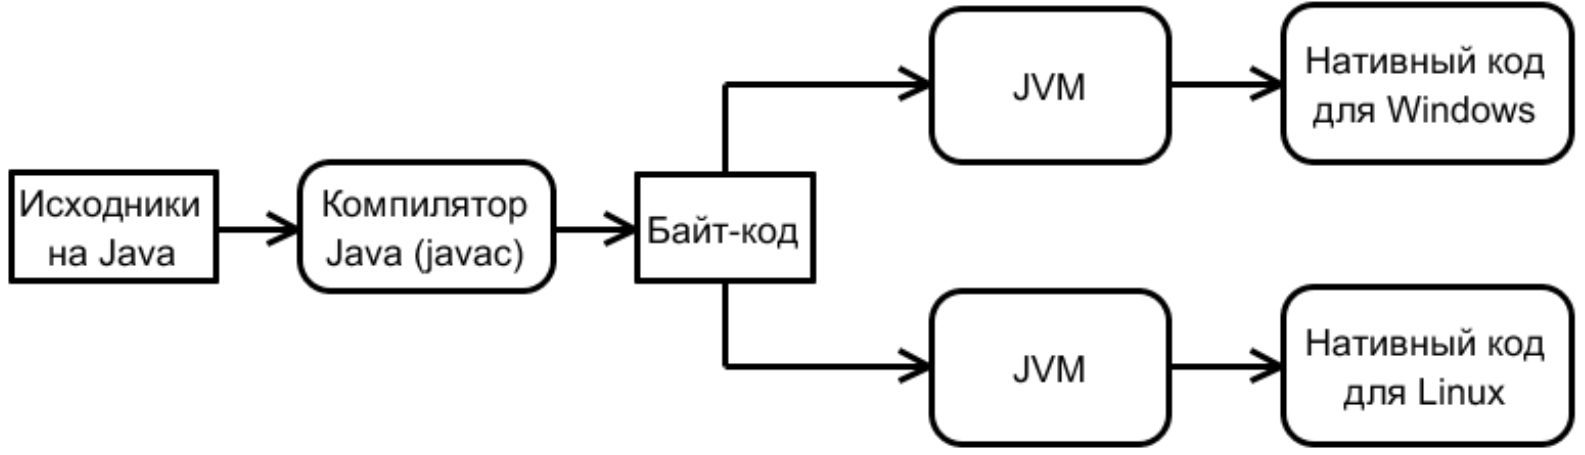
\includegraphics[width=0.8\textwidth]{javaCompiling.png}
	\end{center}
	\caption{Исполнение программы на Java.}
	\label{figure1}
\end{figure}

За такое удобство приходится платить падением скорости работы программы --- ведь интерпретировать инструкцию гораздо дороже, чем просто исполнить её на процессоре. Но существующие Java-машины обычно довольно умные и используют продвинутые техники оптимизации, например Just In Time-компиляцию (это когда последовательность инструкций переводится в машинный код прямо в процессе выполнения программы, а затем запоминается для последующего использования). Многие Java-машины умеют также оптимизировать код на лету, получая данные для оптимизации во время работы программы. Есть и аппаратные реализации Java-машин --- на них Java-приложения могут работать в реальном времени. Вообще, Java-машин очень много, от разных производителей, они предназначены для разных задач --- бывают встроенные в браузеры Java-машины, бывает Java-машина, распространяемая самой Sun вместе со средствами разработки Java, есть Java-машины для мобильных телефонов, карманных компьютеров, и т.д. Следует отметить, что виртуальную машину в качестве среды выполнения использует далеко не только Java --- программы на .NET тоже исполняются .NET-машиной, идея виртуальной машины была предложена ещё Виртом для языка Паскаль. Кстати, важным достоинством виртуальной машины является то, что в её байт-код можно компилировать из сразу нескольких исходных языков, например, в код .NET-машины можно компилировать программы на C\#, C++, Delphi, F\# и т.д., в код Java-машины тоже не одну только Java --- есть ещё языки, типа Scala или Kotlin, ориентирующиеся на Java-машину как среду выполнения, или Ada --- которая имеет компилятор в байт-код Java помимо нативного кода.

Следующим важным отличием Java от С++ является сборка мусора. В С++ надо было следить за выделением памяти --- память, выделенную в куче, надо было освобождать вручную. В Java выделять память надо, а освобождать --- нет, это сделает сама Java-машина, точнее, сборщик мусора (garbage collector). Java-машина следит за тем, на какие области памяти ссылается программа, и если есть выделенная область памяти, на которую не ссылается больше никто, она её удалит. Опять же, это не особенность Java, .NET поступает так же, а сама идея сборки мусора предлагалась ещё в Lisp, в 1959. Кстати, обратите внимание, что наличие сборщика мусора --- это не повод радостно забить на память и выделять объекты на куче пачками, иначе довольно быстро начнутся проблемы с постоянными вызовами сборщика мусора (а он обычно работает небыстро), фрагментацией памяти и т.д., в общем, за памятью надо следить столь же аккуратно, как и в С++, только несколько меньше ручной работы. Плохие новости, кстати, в том, что в Java почти всё выделяется на куче (в C++ программист сам может принимать решение, на стеке или на куче выделять память под тот или иной объект, в Java решение принято раз и навсегда разработчиками языка). Сборщик мусора по большей части предполагает остановку всего приложения и запуск собственно сборки мусора, которая должна просмотреть граф ссылок объектов в памяти, и хотя применяются разные крутые оптимизации, надо понимать, почему лишний раз выделять память плохо (и почему в C++ сборки мусора нет) --- если программа управления крылатой ракетой решит, что ей надо пособирать мусор и заморозить исполнение на несколько десятков миллисекунд, последствия могут быть не очень желательными.

Ещё из концептуальных отличий Java от C++ важны следующие.

\begin{itemize}
	\item В Java (как и во многих остальных современных языках) практически всё является объектом. Например, массивы --- это объекты класса-наследника класса Object (в Java, кстати, все классы наследуют от Object), даже числа, хоть и сами не объекты (они Value Types), приводятся к объектам так называемых обёрточных классов, причём автоматически.
	\item В отличие от C++, где элементарные типы платформозависимы, в Java размер элементарного типа фиксирован спецификацией. То есть, например, int всегда имеет размер 32 бит, long всегда 64 бит (для сравнения, в современном C++ на x86 и x64 int и long --- это одно и то же).
	\item В Java, в отличие от C++, адекватная система модулей, поскольку нет препроцессора и странной системы include-ов. В Java в программе можно использовать имена из любого места кода программы и из любой библиотеки, подключенной к проекту, при этом ничего специально писать не надо. Ну, если использовать полностью квалифицированные имена (вы же знаете, что такое квалифицированные имена и неймспейсы в C++?). Роль неймспейсов в Java играют пакеты (package), отличие в том, что Java довольно фанатично к ним относится --- внутри одного файла может быть только один пакет, причём структура пакетов должна в точности соответствовать структуре папок на диске (отклонение от этого правила --- ошибка компиляции). Например, пакет ru.qreal.kernel должен лежать в папке ru, внутри которой подпапка qreal, внутри которой подпапка kernel. Роль using namespace в Java играет ключевое слово import, роль namespace --- ключевое слово package. Кстати, по стайлгайду пакеты принято именовать, начиная с доменного имени организации-автора пакета, записанного в обратном порядке. Например, если у вас есть домен qreal.ru, то все ваши пакеты лучше именовать ru.qreal.<имя пакета, может быть тоже с подпакетами>. Почему так --- доменные имена глобально уникальны (это обеспечивается службой DNS), так что такая схема именования гарантирует отсутствие конфликтов имён.
	\item Java, как и любой уважающий себя managed-язык (то есть компилирующийся в байт-код), хранит в скомпилированной программе довольно много информации о её статической структуре, которой можно пользоваться во время выполнения. Например, каждый объект имеет ссылку на свой класс, и может спросить, например, своё имя и список своих методов. В C++ ничего такого нет, вся такая информация не переживает компиляции. Это несколько увеличивает требуемый программе объём памяти, но всякие штуки типа плагинов можно реализовать ``прямо из коробки'', да и, например, системы модульного тестирования писать на Java гораздо проще. Библиотека модульного тестирования может сама найти и запустить модульные тесты, практически без помощи программиста. Ещё, кстати, есть такая вещь, как атрибуты, это вообще произвольная информация, которой может быть помечен узел абстрактного синтаксического дерева программы. Они, в совокупности с возможностью генерировать байт-код ``на лету'', позволяют писать полиморфный код и вообще делать всякие ужасные вещи (что активно используется в аспектно-ориентированной парадигме программирования). На C++ такое не сделать.
	\item В Java 8 наконец появились лямбда-функции, функциональный интерфейс для работы с коллекциями (функции типа map, fold, filter и т.д.). В C++ оно тоже появилось, причём на три года раньше, чем в Java, тут надо отдать C++ должное. К тому же, в Java лямбда-функции реализованы довольно неудобно, но лучше так, чем никак.
	\item В Java по историческим причинам, связанным с необходимостью поддержки обратной совместимости, очень странная поддержка шаблонов. Она радикально отличается от C++ (ну, C++ в плане шаблонов вообще особый язык, и ещё неизвестно, хорошо это или плохо). В Java шаблоны называются генериками и они концептуально более честные, чем в C++ (реализуют ``честный'' параметрический полиморфизм, то есть для разных инстанциаций одного шаблона исполняется один и тот же код, в отличие от C++, где каждая инстанциация --- это свой отдельный кусок машинного кода, что делает шаблоны C++ больше похожими на макроподстановку, чем на шаблоны). Проблема генериков в Java в том, что в ранних версиях Java их не было, а сохранить обратную совместимость со старыми Java-машинами (некоторые из которых реализованы аппаратно) было надо, поэтому в байт-коде Java до сих пор понятия ``генерик'' нет. Вот так, шаблон --- структура времени компиляции, во время выполнения программа вообще ничего не знает про шаблоны, что приводит к довольно забавным концептуальным проблемам типа невозможности создать объект параметра-типа.
\end{itemize}

Если что-то из списка выше было непонятно, про все подобного рода вещи я буду рассказывать дальше, так что можно относиться к этому как к краткому содержанию следующих серий.

\section{Типы в Java}

Для начала небольшое ``теоретичекое'' введение про систему типов языка. Вот таблица с числовыми типами:

\begin{tabu} {| X[0.3 l p] | X[1 l p] | X[0.2 l p] |}
	\tabucline-
	Тип       & Значения                                                                              & Размер  \\
	\tabucline-
	\everyrow{\tabucline-}
	$byte$    & $-2^7..2^7-1 (-128..127)$                                                             & 8 бит   \\
	$short$   & $-2^15..2^15-1 (-32768..32767)$                                                       & 16 бит  \\
	$int$     & $-2^31..2^31-1$                                                                       & 32 бит  \\
	$long$    & $-2^63 .. 2^63-1$                                                                     & 64 бит  \\
	$float$   & $-3.4028235E+38..-1.4E-45$ \newline и $1.4E-45..3.4028235E+38$                        & 32 бит  \\
	$double$  & $-1.7976931348623157E+308..-4.9E-324$ \newline и $4.9E-324..1.7976931348623157E+308$  & 64 бит  \\
\end{tabu}

Как говорилось выше, типы стандартизованы, поэтому их размер и диапазон значений не зависят от конкретной платформы. Ещё можно обратить внимание, что нет беззнаковых числовых типов.

Несколько более непривычно для C++-программистов то, что все типы вообще делятся на ссылочные типы и типы-значения (или, как их называют в Java, примитивные типы). Разница между ними в том, что ссылочные типы всегда хранятся на куче и передаются по ссылке, значения примитивных типов всегда и хранятся, и передаются по значению. То есть, переменная ссылочного типа --- это ссылка на участок памяти в куче, где лежит значение этого типа, ссылка --- это просто указатель, который нельзя разыменовывать. И нет нужды, потому что обращение к полю и вызов метода всегда выполняются с разыменованием (то есть оператор . в Java аналогичен оператору -> в C++), присваивание и сравнение выполняются для самой ссылки, а не для её значения, а больше ничего делать со ссылками и нельзя. Да, это важно --- в Java нет перегрузки операторов, поэтому присваивание и сравнение выполняются всегда с самой ссылкой. \mintinline{java}|Object b = a;| не  копирует значения полей из a в b и не вызывает конструктор копирования (в Java такого просто нет), а делает так, чтобы b ссылалась на тот же объект, что и a. Со сравнением то же самое, поэтому, например, 

\begin{minted}{java}
String a = "1";
String b = "1";
System.out.println(a == b);
\end{minted}

вполне может выдать false (на самом деле нет, потому что есть такая вещь, как интернирование строк, но идею вы поняли). Строки надо сравнивать только методом equals().

Какие типы примитивные, а какие ссылочные, за нас решили авторы языка (в отличие от C++). Примитивные типы --- это \mintinline{java}|byte, short, int, long, float, double, boolean, char|. Ссылочные типы --- это всё остальное: массивы, классы (в том числе строки и типы-обёртки), интерфейсы, перечисления, аннотации. У каждого типа есть значение по умолчанию, и все поля при создании объекта получают эти самые значения по умолчанию --- 0 для числовых типов, false для булевого типа, '\\0' для char, null для всех ссылочных типов (да, даже для строк). На самом деле, Java-машина при выделении памяти под объект просто заполняет всю память нулями всегда, так что неинициализированных переменных в Java не бывает. Она так не делает при инициализации кадра стека, поэтому могут быть неинициализированные локальные переменные, но использование неинициализированной локальной переменной --- это ошибка компиляции (опять-таки, в отличие от C++). Семантику инициализации надо чётко себе представлять, иначе можно получить NullPointerException на ровном месте:

\begin{minted}{java}
public static void main(String[] args) {
    int[][] matrix = new int[10][];
    if (matrix[5].length == 0) {
        System.out.println("Never get here");
    }
}
\end{minted}

Это опять-таки местами может быть непривычно C++-программистам, где \mintinline{cpp}|vector<vector<int>>| никакой дополнительной инициализации не требует.

Выше несколько раз упоминались типы-обёртки без всяких пояснений, пришла пора рассказать, что это. Тип-обёртка (Wrapper type) --- это класс, соответствующий примитивному типу, причём это соответствие поддерживается компилятором, так что значение примитивного типа при необходимости приводится к значению типа-обёртки и обратно. Такое приведение, кстати, называется \textbf{boxing} --- для приведения от примитивного типа к классу, и \textbf{unboxing} --- для приведения от класса к примитивному типу. Нужно это в ситуациях, когда у нас есть значение примитивного типа и мы хотим его передать туда, где ожидается объект (например, когда вы узнаете страшную правду про генерики в Java, будет понятно почему, но \mintinline{java}|LinkedList<int>| не скомпилится, скомпилится \mintinline{java}|LinkedList<Integer>|, и поэтому при добавлении числа в список чисел каждый раз выполняется boxing). Зато обёрточные типы имеют разные полезные методы, например, разбор строки: \mintinline{java}|int ololo = Integer.parseInt("239");|.

Обёрточные типы обычно называются так же, как примитивные типы, которые они оборачивают, только с заглавной: \mintinline{java}|byte| --- \mintinline{java}|Byte|, \mintinline{java}|short| --- \mintinline{java}|Short|. Однако, чтобы всех запутать, есть два исключения: \mintinline{java}|char| --- \mintinline{java}|Character|, \mintinline{java}|int| --- \mintinline{java}|Integer|. Ну и это вообще не обязательно знать, и, я думаю, даже вредно знать после первой пары, но есть один известный прикол, связанный с обёрточными типами: \mintinline{java}|Integer.valueOf(127) == Integer.valueOf(127)|, но \mintinline{java}|Integer.valueOf(128) != Integer.valueOf(128)|. Единственно правильный способ вручную обернуть примитивный тип в обёрточный --- это вызвать статический метод valueOf, который вернёт объёкт, содержащий число, при этом в целях оптимизации Java-машина кеширует числа от -128 (кажется) до 127, дабы не возвращать каждый раз новый объект и не выделять под него память. Поэтому \mintinline{java}|Integer.valueOf(0)| ... \mintinline{java}|Integer.valueOf(127)| возвращает закешированные объекты, которые всегда ссылочно равны, а вот \mintinline{java}|Integer.valueOf(128)| и далее честно вызывают конструктор Integer и возвращают новые объекты, каждый из которых не равен другому ссылочно. А поскольку в Java нет перегрузки операторов, == ведёт себя так странно. Это любимый вопрос на собеседованиях по Java, типа как ``Что такое виртуальное наследование'' на собесседованиях по C++ --- в реальной жизни нафиг не нужно, но позволяет отличить Посвящённых от шкальников.

\section{Демонстрация}

<дальше демострация на проекторе, запускаем IntelliJ IDEA>

Теперь можно перейти к техническим деталям. Создаём новый проект типа ``Java Hello world'' Получаем что-то такое:

\begin{minted}{java}
public class Main {
    public static void main(String[] args) {
        System.out.println("Hello World!");
    }
}
\end{minted}

Что мы тут видим: во-первых, работающая программа на Java, как и на любом другом ОО-языке, представляет собой набор объектов, взаимодействующих друг с другом. Тип объекта --- это класс. При этом в Java, в отличие от C++, нет свободных функций, то есть вообще весь код должен быть написан в каком-нибудь классе. Разделения на хедеры и cpp-шники в Java нет, всё, что относится к одному классу, пишется в одном файле, с расширением .java. Считается хорошим тоном поддерживать соответствие ``один файл --- один класс'' (это даже по большей части проверяется  компилятором). При этом каждый класс относится к некоторому пакету, пакеты могут быть вложенными. Если имя пакета не задано, класс относится к пакету по умолчанию, который нельзя импортировать, так что использовать его не рекомендуется, давайте сразу же укажем пакет:

\begin{minted}{java}
package com.example.java;

public class Main {
    public static void main(String[] args) {
        System.out.println("Hello World!");
    }
}
\end{minted}

Пакеты предназначены для организации классов и отвечают за видимость классов друг другу, кроме того, одноимённые классы из разных пакетов можно различить, указывая квалифицированное имя класса: <имя пакета>.<имя класса>. Всё это очень похоже на пространства имён C++. Как я уже говорил, структура вложенности пакетов должна соответствовать структуре вложенности папок в файловой системе, то есть пакету соответствует папка с исходниками. Первой строкой в файле должна быть конструкция package, которая говорит, к какому пакету относится всё, что в этом файле описано. В принципе, package можно не писать, тогда содержимое файла попадёт в пакет по умолчанию, но это невежливо.

Дальше мы видим объявление класса Main. Модификатор доступа public говорит компилятору, что этот класс должен быть виден (то есть, его можно использовать) и в других пакетах. Если этого не написать, класс будет видим только в своём пакете.

Внутри фигурных скобок находятся объявления полей и методов класса, вложенных классов, перечислений и т.д. В нашем случае в классе есть только метод main, который во-первых, public --- то есть относится к интерфейсу класса и может быть использован другими классами, которым виден класс Main, во-вторых он static --- то есть он является методом класса, в противоположность обычным методам, которые относятся к конкретному объекту. Всё как в  С++, разве что модификаторы видимости надо писать перед каждым полем и методом. Кроме того, другие соглашения касательно умолчаний, в Java, если модификатор видимости не указан, принимается по умолчанию пакетная видимость. Поэтому модификаторы видимости лучше указывать явно, метод, который мог бы быть private, но из-за отсутствия модификатора доступа имеет пакетную видимость --- нарушение инкапсуляции и может стать причиной незачтённой домашки.

Продолжим смотреть на код. В отличие от С++ ``функция'' main является методом класса, кроме того, не возвращает код возврата и принимает только массив аргументов (в C++ она вынуждена принимать ещё и количество аргументов, в Java массив сам знает свой размер, как vector в C++, так что main принимает один параметр). Как и в C++, это список аргументов командной строки, переданных программе, но в отличие от C++ аргументы не содержат исполняемого файла программы, потому что у Java понятие ``исполняемый файл'' весьма растяжимо. При желании эту информацию можно вытащить рефлексией.

Дальше стоит вызов метода println статического объекта out класса System. У out есть ещё много всяких полезных методов, например, метод форматированного вывода, типа сишного printf: System.out.format("\%d", 239);, ну и просто print, который делает то же самое, что и println, но строку не переводит. Заметьте, println может выводить всё без всякой форматной строки.

Синтаксис тел методов весьма похож на C++, так что скорее всего получится просто сесть и начать писать код так, будто бы это был С++. Например, цикл for:

\begin{minted}{java}
for (int i = 0; i < 300; ++i) {
    System.out.println("Hello World!");
}
\end{minted}

Функции делаются, например, так:

\begin{minted}{java}
private static int factorial(int n) {
    if (n == 1) {
        return 1;
    }

    return n * factorial(n - 1);
}
\end{minted}

и вызываются так:

\begin{minted}{java}
public static void main(String[] args) {
    System.out.format("Hello, %d", factorial(5));
}
\end{minted}

--- это нужно писать в классе Main на том же уровне, что и функция main. Компилятор многопроходный, поэтому ему плевать, выше или ниже функции main описана наша функция (опять-таки, в отличие от C++).

Для объявления локальных переменных есть var, это аналог C++-ного auto.

Массивы: 

\begin{minted}{java}
int[] a = new int[10]; 
\end{minted}

(обратите внимание на странное положение квадратных скобок)

\begin{minted}{java}
for (int i = 0; i < a.length; ++i) {
   a[i] = i;
}
\end{minted}

Структур в Java нет, их роль играют классы, что довольно грустно с точки зрения производительности и многословности кода. Пример описания класса:

\begin{minted}{java}
public static class Point {
   public int x;
   public int y;
}
\end{minted}

Есть типы-перечисления:

\begin{minted}{java}
enum Grade {
   EXCELLENT,
   GOOD,
   SATISFACTORY
}
\end{minted}

Они больше похожи на enum class из C++11, в том смысле, что они ``сами себе пространство имён'' (кстати, в Java не надо точки с запятой в конце определения), и использовать их надо примерно так:

\begin{minted}{java}
Grade grade = Grade.EXCELLENT;
if (grade == Grade.SATISFACTORY) {
   System.out.println("Fail");
}
\end{minted}

Константы задаются с помощью ключевого слова final --- если в классе: \mintinline{java}|private final double PI = 3.14;|, если в методе --- без модификатора доступа, просто \mintinline{java}|final double PI = 3.14;|

Всякие математические штуки находятся в классе Math. Например, Math.cos(1);

Ещё можно выводить не в консоль, а сразу на графическое окошко. Окошко --- это класс, описанный в пакете javax.swing. Для того, чтобы его можно было использовать, надо сначала импортировать пакет, написав под package, но до public class Main строку import javax.swing.*; --- импортировать все классы из пакета javax.swing (типа С++ного using namespace). Потом в коде программы можно будет написать что-нить вроде

\begin{minted}{java}
JOptionPane.showMessageDialog(null, "Ololo!");
\end{minted}

Можно было сразу написать import javax.swing.JOptionPane; - так мы импортируем конкретно нужный класс, и это считается хорошим тоном. Можно было вообще импорт не писать, а писать в коде javax.swing.JOptionPane.showMessageDialog(null, "Ololo!");  --- по аналогии с C++ным std::string или using namespace std; и затем string;

Так же примерно можно сделать окошко для ввода:

\begin{minted}{java}
String test = javax.swing.JOptionPane.showInputDialog("Ololo!");
\end{minted}

С чтением из консоли дело обстоит несколько хуже: в пакете java.io есть классы BufferedReader и InputStreamReader. Считать строку из консоли можно, например, так:

\begin{minted}{java}
BufferedReader in = new BufferedReader(
    new InputStreamReader(System.in));
try {
   String input = in.readLine();
} catch (Exception e) {
    System.out.println("Что-то пошло не так");
}
\end{minted}

ну или написать в функции main, что она throws Exception. Про исключения в Java потом будет рассказано отдельно, они несколько отличаются от C++-ных исключений, и главное, компилятор Java следит, что все бросаемые методом исключения задекларированы (ну, не все, но про это потом). Хорошая новость в том, что IDEA умеет автоматически сгенерить либо try-catch, либо конструкцию throws, которая, собственно, декларирует кидаемые методом исключения. Ещё, кстати, с какого-то момента так писать будет нельзя, потому что правильнее вот так, но про это на следующей неделе:

\begin{minted}{java}
try (BufferedReader in = new BufferedReader(
    new InputStreamReader(System.in))) 
{
   String input = in.readLine();
   ...
} catch (Exception e) {
   ...
}
\end{minted}

\section{Инструменты}

Что скачать, чтобы всё было --- есть дистрибутив JDK 11, лежит на \url{https://www.oracle.com/technetwork/java/javase/downloads/jdk11-downloads-5066655.html}. Обратите внимание, есть JDK (Java Development Kit) --- это Java-машина, компилятор, стандартная библиотека плюс некоторое количество полезных утилит. Есть JRE (Java Runtime Environment) --- это только Java-машина плюс скомпилированная стандартная библиотека, должна быть на целевом устройстве для того, чтобы Java-программы на нём работали. Короче, JDK для программистов, JRE для пользователей, вам нужен JDK. Причём, JDK 11, по умолчанию может скачаться JDK 8, но мы не пользуемся legacy-технологиями. Чтобы всё работало из консоли, надо прописать путь до копилятора javac в PATH (под Windows он обычно лежит в Program Files\\Java\\jdk-<номер версии>\\bin) и прописать переменную окружения JAVA\_HOME (это Program Files\\Java\\jdk-<номер версии>). Под Linux и подобными системами всё примерно так же, только пути другие, но тут, надеюсь, любители конкретных дистрибутивов сами разберутся. Если работа с переменными окружения незнакома, пишите.

Из консоли программировать --- такое себе удовольствие (хотя в JDK недавно появилась утилита jshell --- CLI-интерпретатор Java, чтобы играться с языком прямо в консоли без компилятора). Настоятельно рекомендуется поставить IDE, бесплатная для студентов и очень годная среда разработки IntelliJ IDEA доступна по ссылке \url{https://www.jetbrains.com/student/}. В принципе, ещё в мире Java популярны среды Eclipse и NetBeans, но скорее по историческим причинам. Домашки можно писать под чем угодно (мало ли вы фанат Eclipse), но показывваться всё будет на примере IDEA.

Если вы выбрали IDEA в качестве среды разработки, то не поленитесь сразу же прописать .gitignore для репозитория с домашками так, чтобы туда попадали только нужные файлы (про .gitignore будет подробно на следующей неделе, так что кто не умеет, следите пока вручную за тем, что выкладываете). Для Java + IDEA надо выкладывать файлы .java и содержимое папки .idea, кроме workspace.xml, usage.statistics.xml, tasks.xml. Файлы .class выкладывать нельзя (домашка будет сразу отправлена на доработку). Решения домашек должны коммититься в git, пушиться в репозиторий на GitHub в отдельную ветку, из этой ветки должен открываться пуллреквест в мастер, и ссылку на этот пуллреквест надо сдать в качестве решения на HwProj, только после этого оно будет проверено. Для всех домашних работ предлагается завести один репозиторий (они будут не очень большими и их будет много, так что захламлять свой аккаунт кучей репозиториев не стоит), задачи раскладывать по папкам внутри репозитория. Каждая задача --- отдельный проект в IDEA. Решение каждой задачи надо начинать с отведения новой ветки от мастера и создания в этой ветке новой папки и нового проекта в ней. Когда задача будет проверена, к ней, скорее всего, будут замечания --- чтобы их поправить, надо переключиться на ветку с задачей (кстати, никто не запрещает иметь несколько разных папок со склоненным репозиторием, для разных задачек), поправить замечания там, закоммитить в эту же ветку и запушить. После чего ещё раз приложить ссылку на тот же пуллреквест (в который добавятся ваши новые коммиты) на HwProj. Кто без идей, что всё это значит, делайте как умеете, на следующей неделе будет подробно про git.

\subsection{Работа из консоли}

Даже если у вас есть IDE, необходимо уметь собирать программы и из консоли (например, если вам надо будет компилить что-то по ssh на удалённом сервере, или для того, чтобы уметь вручную настроить сборку в системе непрерывной интеграции). Для этого используется компилятор javac:

\begin{minted}{text}
javac MyClass.java YetAnotherClass.java
javac -d classes MyClass.java
javac -classpath classes;library.jar -d classes MyClass.java
\end{minted}

Ключ -d позволяет задать папку, куда сложить результат (примерно как -o в gcc для C++, но есть одно важное различие). Ключ -classpath (или -cp) говорит компилятору, где брать библиотеки, которые использует ваша программа (что-то вроде ключей -l и -L в gcc). CLASSPATH по умолчанию содержит папку со стандартной библиотекой, поэтому её указыввать явно никогда не нужно, и если у вас не находится, например, String, то дело не в CLASSPATH, а, скорее всего, в том, что у вас JAVA\_HOME не прописана.

Вообще понятие CLASSPATH для Java очень важно --- оно используется не только при компиляции, но и при работе программы, и используется для того же --- для загрузки классов и библиотек, которые программа использует. CLASSPATH задаётся как набор путей или JAR-файлов, разделённых ``;'' в Windows или через ``:'' во всём остальном (как PATH), по умолчанию это текущая папка. К CLASSPATH также добавляются пути к библиотекам из JAVA\_HOME. Кстати, ``библиотека'' в Java --- это JAR-файл, который по сути папка со скомпилированными в байт-код классами, запакованная zip (кстати, поэтому её можно легко распаковать и посмотреть содержимое). Помимо собственно байт-кода там ещё лежит некоторое количество метаинформации (манифест) и необходимые коду ресурсы (картинки, тексты и т.д.).

Собственно, запуск из консоли выполняется командами java или javaw (разница между ними в том, что javaw не открывает окно консоли, поэтому используется для приложений с GUI). Например, вот так можно запустить программу:

\begin{minted}{text}
java MyClass
\end{minted}

Или:

\begin{minted}{text}
java -classpath classes\_dir;library.jar MyClass
java -jar library\_with\_main\_class.jar
\end{minted}

Обратите внимание, Java при компиляции не генерит .exe или какой-либо другой исполнимый файл, который можно просто запустить и исполнить (как в C++), что логично, потому что для разных ОС формат исполнимых файлов разный, а программа должна запускаться повсюду. Более того, в Java программа обычно даже не собирается в один какой-то файл, который можно отдать виртуальной машине на исполнение (в отличие от, скажем, .NET). Виртуальной машине Java передаётся полностью квалифицированное имя класса, который нужно запустить, и CLASSPATH, где она может найти все остальные классы, нужные для работы. Чтобы было можно запустить класс, он должен иметь метод \mintinline{java}|public static void main(String[] args)|, именно с такой сигнатурой. Это имеет один приятный побочный эффект --- в программе может быть сколько угодно точек входа, хоть каждый класс можно сделать запускаемым (и некоторые Java-разработчики в былые времена это использовали, чтобы писать каждому классу что-то вроде юнит-тестов, но это совершенно не нужно, потому что есть библиотеки юнит-тестирования). Ключ -jar говорит взять JAR-архив, посмотреть в его манифест и найти запускаемый файл, который в нём прописан. Поскольку это доставляет минимум боли пользователю, типичный способ распространения десктопного Java-приложения --- это как раз JAR, в котором лежит всё, что нужно для исполнения программы.

Ещё раз обращу внимание, что в командной строке указывается именно имя класса, а не имя файла или что-то ещё. И оно должно быть полностью квалифицированным, то есть помимо имени класса содержать и полное имя пакета, в котором он содержится (например, com.example.MyClass). Ещё есть куча опций для виртуальной машины, вплоть до максимального объёма выделяемой программе памяти. Рекомендую посмотреть документацию на предмет интересных ключей. Запускать из консоли надо уметь, и кажется, это потребуется в одной из контрольных, поэтому тут так подробно про это рассказывается. Хорошая новость в том, что в Java очень развиты системы сборки, они могут сделать всё за вас --- и собрать stand-alone JAR-ник, и даже его правильно запустить. Про системы сборки буквально на следующей паре.

\subsection{Некоторые тонкости IntelliJ IDEA}

Некоторые советы по поводу использования IDEA:

\begin{itemize}
	\item Есть отдельно меню File -> Settings и отдельно File -> Project Structure. Settings --- это в основном настройки самой среды, типа настроек редактора и путей до разных инструментов. Но, чтобы всех запутать, там есть и настройки, специфичные для проекта, например, использование процессоров аннотаций (впрочем, в первом модуле они нам не понадобятся). Project Structure же --- это настройки проекта. Тут указывается версия языка, версия JDK (это разные вещи, можно использовать JDK 11, но задать уровень языка Java 7, тогда компилятор будет ругаться на var-ы и прочие полезные вещи, появившиеся недавно). Тут же указывается структура проекта --- какие папки IDEA считает папками с кодом, какие --- с тестами, какие --- с ресурсами, какие вообще игнорирует при сборке. Если у вас код написан правильно, но IDEA вообще ничего не компилит (и даже не пытается), имеет смысл посмотреть сюда. IDEA компилит только папки, отмеченные как Sources или Tests. Тут же указываются сторонние библиотеки, подключенные к проекту. Обратите внимание, что всё это настройки конкретно проекта IDEA и на консольную сборку они никак не влияют. Когда вы используете систему сборки, то IDEA может импортировать настройки из файла конфигурации сборки в проект, но после этого настройки могут разойтись, так что возможна (хотя и очень редка) ситуация, когда из консоли собирается, а из IDE-нет. В таком случае не надо пугаться, надо просто импортировать настройки сборки ещё раз (в самом запущенном случае --- удалить папку .idea и импортировать весь проект заново).
	\item Справа вверху --- конфигурации запуска. Там можно настроить, например, параметры командной строки. Конфигурация запуска создаётся автоматически, когда вы кликаете на зелёную стрелочку рядом с запускаемым методом, потом её можно редактировать.
	\item Основные хоткеи --- Alt-Enter (``сделать, чтобы всё было правильно'', встаём курсором на место с ошибкой и жмём), Ctrl-B (перейти к объявлению), Shift-F9 (Debug), Shift-F10 (Run), отладка: F9 (исполнить дальше), F8 (Step Over), F7 (Step Into), Shift-F8 (Step Out). Вообще, не поленитесь посмотреть хоткеи по меню, это может быть очень полезно на контрольной.
\end{itemize}

\section{Стайлгайд}

Стиль кодирования в Java стандартизован (опять-таки в отличие от С++), потому что Sun ещё в конце 90-х не поленилась написать подробный документ и навязывать его сообществу разработчиков. Тот документ в последний раз обновлялся, кажется, в 1998 году, так что мы будем руководствоваться стилем кодирования от Google: \url{https://google.github.io/styleguide/javaguide.html}, за единственным исключением --- для отступа используется 4 пробела, а не 2 (это, наверное, неправильно, но 4 пробела используют все, кроме Google). Поскольку стиль кодирования стандартизован, сообщество весьма фанатично его придерживается, так что и мы будем --- решения, не соответствующие стилю кодирования, будут отправляться на переделку. В IDEA по умолчанию стиль кодирования такой, какой нужен, поэтому следовать ему не так сложно, как кажется --- просто позволяйте IDEA форматировать ваш код и не игнорируйте предупреждения.

На что стоит особенно обратить внимание:

\begin{itemize}
	\item Стиль именования camelCase (со строчной) используется для имён методов, полей класса, параметров, локальных переменных. Стиль CamelCase (с заглавной) используется для типов (классов, интерфейсов, перечислений и т.д.), КАПС\_ДЛЯ\_КОНСТАНТ (в том числе, элементов перечисления). Интерфейсы в Java не имеют специальных префиксов (в отличие, например, от .NET с его IEnumerable и т.п.), поля тоже префиксами и суффиксами не выделяются.
	\item Стиль именования пакетов --- это DNS-имя организации, разрабатывающей пакет, записанное наоборот (то есть если вы владеете доменным именем example.com, то префикс имени пакета --- com.example) плюс, собвственно, имя пакета, записанное строчными буквами без разделителей (например, com.example.mycoolpackage).
	\item Стиль расстановки фигурных скобок --- ``Египетские'' (так же известны, как стиль K \& R):
		\begin{minted}{java}
public static void myMethod() {
    for (int i = 0; i < 300; ++i) {
        System.out.println("Cthulhu fhtagn!");
    }
}
		\end{minted}
		Скобки ставятся вокруг тела оператора даже если в оном теле только один оператор, обратите внимание. Даже если это if что-то-там return.
	\item Инкапсуляция. Поля, методы и всё-всё-всё должны иметь минимально возможную видимость, при которой программа всё ещё компилится. Локальные переменные должны иметь минимальную область видимости (то есть если переменная используется только внутри цикла, её надо там и объявлять). Умолчания в Java не очень удобные (пакетная видимость для членов класса, например), так что модификаторы видимости почти всегда надо писать явно. Почти --- потому что иногда пакетная видимость всё-таки бывает полезна (хотя часто это может оказаться плохой идеей).
	\item Нужны комментарии к каждому классу (интерфейсу, перечислению и т.д.) и каждому public-методу. Комментарии к полям и private-методам опциональны, но желательны. Есть стандартная система генерации документации по комментариям в коде JavaDoc (кстати, документация к стандартной библиотеке сгенерирована именно ей), комментарии надо писать в её стиле. Очень рекомендуется иногда генерировать JavaDoc-и (благо это делается парой кликов в IDEA) и смотреть, что получилось.
\end{itemize}

В IDEA JavaDoc запускается через меню Tools, Generate JavaDoc. JavaDoc-комментарии пишутся над комментируемой сущностью и имеют вид \mintinline{java}|/** текст комментария */|. Комментарии внутри методов игнорируются, так что такие комментарии имеет смысл писать как обычные, а не как JavaDoc-и, чтобы не смущать читателя. Комментарии начинаются с общего описания, за которым могут идти тэгии, содержащие дополнительную информацию. Например,

\begin{minted}{java}
/** Praises the Great Cthulhu.
 *  @param times how many times Great Cthulhu shall be praised
 *  @throws RuntimeException when finished */
public static void myMethod(int times) {
    for (int i = 0; i < times; ++i) {
        System.out.println("Cthulhu fhtagn!");
    }

    throw new RuntimeException();
}
\end{minted}

Если подробности малоинформативны или дедлайн через 20 минут, можно писать однострочные комментарии:

\begin{minted}{java}
/** Praises the Great Cthulhu. */
public static void myMethod(int times) {
    for (int i = 0; i < times; ++i) {
        System.out.println("Cthulhu fhtagn!");
    }

    throw new RuntimeException();
}
\end{minted}

Можно вообще не писать комментарии в случаях, если назначение метода самоочевидно (но только если оно абсолютно 100\% самоочевидно всем, не только вам). Например, геттеры:

\begin{minted}{java}
public int getValue() {
    return value;
}
\end{minted}

Популярные тэги:
\begin{itemize}
	\item \mintinline{java}|@param имя описание параметра| --- комментарий к параметру метода;
	\item \mintinline{java}|@return описание возвращаемого значения| --- описание того, что метод возвращает;
	\item \mintinline{java}|@exception ИмяКлассаИсключения описание, когда бросается| --- описание ситуации, когда метод бросает исключение, для каждого типа бросаемых исключений;
	\item \mintinline{java}|{@inheritDoc}| --- скопировать документацию к этому методу из класса-предка;
	\item \mintinline{java}|@see| --- ссылка на другой класс, метод или что-то ещё, у чего есть документация.
\end{itemize}

Обращаю внимание, что комментарий должен начинаться с общего описания (иногда есть большой соблазн сразу написать @return, боритесь с этим). Ещё пустые тэги не пишите, даже если их вам услужливо сгенерит среда разработки --- либо уж напишите комментарий, либо удалите их.

\end{document}
